\documentclass{article}
\usepackage{amsmath}
\usepackage{amssymb}
\usepackage{graphicx}
\usepackage{enumitem}
\usepackage[utf8]{inputenc}
\graphicspath{{/home/stephanie/Escritorio/THC/Taller-de-Herramientas-Computacionales/Clases/Latex/Imagenes/}}

\title{\Huge Taller de Herramientas Computacionales}
\author{Stephanie Escobar Sánchez}
\date{20/enero/2019}
\begin{document}
	\maketitle
\begin{center}
	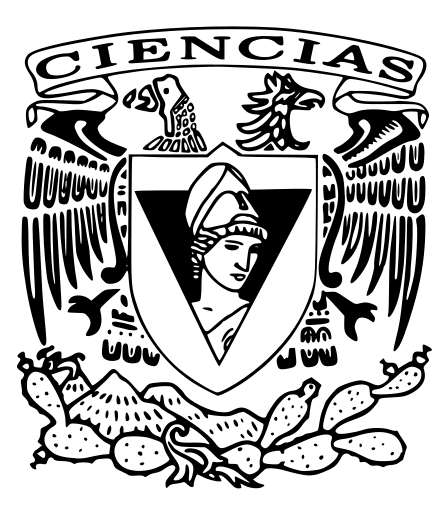
\includegraphics[scale=0.40]{1.png}	
\end{center}
\newpage
\title{\Huge Bitácora clase 7} \\
\\
Comenzamos trabajando con el problema del día anterior, que era definir la función raíz cuadrada a partir de un rectángulo con base x y altura 1, retomamos conceptos sobre dónde son importantes los espacios en python qué es en los bloques, ya que si algo no está en el bloque correcto el programa podría no correr adecuadamente o darnos resultados incorrectos.\\
\\
Primero, es importante definir los datos de entrada, que son los datos que ya sabemos a partir de los cuales vamos a trabajar. Es importante definir bien las variables y saber en qué variable es en donde se va a guardar el resultado para poder pedirlo al final. Primero es importante definir la función, que se compone de condiciones iniciales y cálculos para llegar a un resultado.\\
\\
Otra cosa importante es tener cuidado de no cometer errores, debido a que nos puede quitar mucho tiempo de trabajo, algo importante cuando cometemos un error y no sabemos por qué es conocer cuáles son algunos de los errores comunes y revisar si no hemos cometido alguno de ellos antes de ir directamente al código. Algunos de los errores más comunes es el uso de mayúsculas y minúsculas, muchas veces podemos tener el código muy bien hecho y de repente nos marca un error, debemos fijarnos que todas las letras que definimos sean mayúsculas o minúsculas según las hayamos definido. Otro de los errores tienen que ver con "dedazos" que cometemos cuando escribimos alguna letra de más o de menos y no nos dimos cuenta, también el equivocarnos con los signos, como cambiar un mayor qué por un menor qué o un más por un menos. Es importante también fijarnos que el código esté bien hecho aunque si corra el programa porque si cometimos un error en un signo puede darnos resultados incorrectos y nosotros no saberlo. Una forma de evitar ésto es siempre probarlo con la solución trivial y que ya sabemos el resultado para ver que estén bien cálculos más complejos.\\
\\
El problema de la clase fue definir la sucesión ulam con ayuda de los comandos \textit{if} y \textit{while}:\\
Si x es par x= x/2\\
Si x es impar X= 3x+1 \\
\\
Algo importante es siempre resolver el problema en lápiz y papel para después pasar al código. Finalmente lo resolvimos mediante el código:
\begin{verbatim} 

def ulam (x):
	print (x)		
	while x>1:
	p = x / 2

		if x == 2*p:
		x = x/2
		i=i+1
		print (x)
		else:
			x = 3*x + 1
			i=i+1
		print (x)
		return ('se hizo %d veces' % (i))

\end{verbatim}
La letra i nos sirve como contador cuando ponemos i=0 antes un ciclo while y nos permkite saber cuántas veces se repitió el programa.\\

\end{document}
